%Quote package define
\usepackage{framed}
\definecolor{shadecolor}{RGB}{240,240,240}
\newenvironment{magquote}
  {\begin{shaded*}\itshape\small}
  {\end{shaded*}}


% Article 3
% ====================
% YOUR ARTICLE
% ====================

  
\article{Beyond the Firewall, Threats Never Sleep}{Ferdous Ara Fahima}{June 28, 2025}

\begin{magquote}
 ``There are two types of companies: those that have been hacked, and those who don’t know they have been hacked.'' -- John Chambers   
\end{magquote}



\lettrine[lines=2]{I}{n} an era where our lives are intertwined with technology, cybersecurity stands as the guardian of our digital existence. From personal data to critical infrastructure, the invisible threats lurking in the shadows of the internet are ever-present. Hackers, like skilled predators, exploit the smallest vulnerabilities, turning our reliance on technology into a potential weakness. This article explores the critical landscape of cybersecurity: its necessity, the impact of cyberattacks, and how to protect our digital future.

\begin{figure}[h]
  \centering
  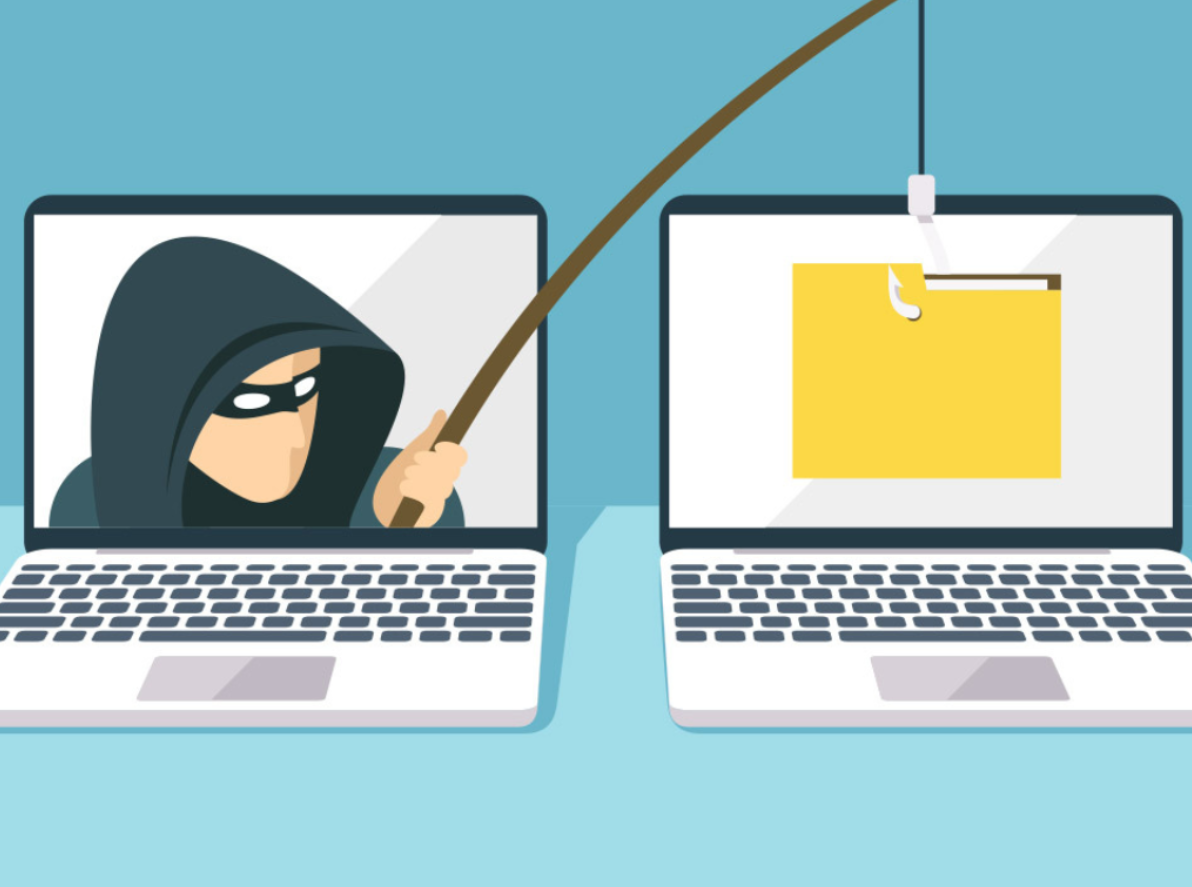
\includegraphics[width=0.45\textwidth]{phishing.png}
  \caption{\textit{Hacker is fishing. Don't be his Hilsha.}}
\end{figure}

\section*{The Digital World: Scale and Stakes}
As of 2025, the global population is around 8.2 billion, with 5.4 billion (66\%) actively using the internet. This massive connectivity fuels innovation but also creates a vast playground for cybercriminals. Every connected device—from smartphones to IoT appliances—is a potential entry point for attacks. A single breach can lead to identity theft, financial loss, or life-threatening disruptions, making cybersecurity an urgent global priority.

\begin{figure}[h]
  \centering
  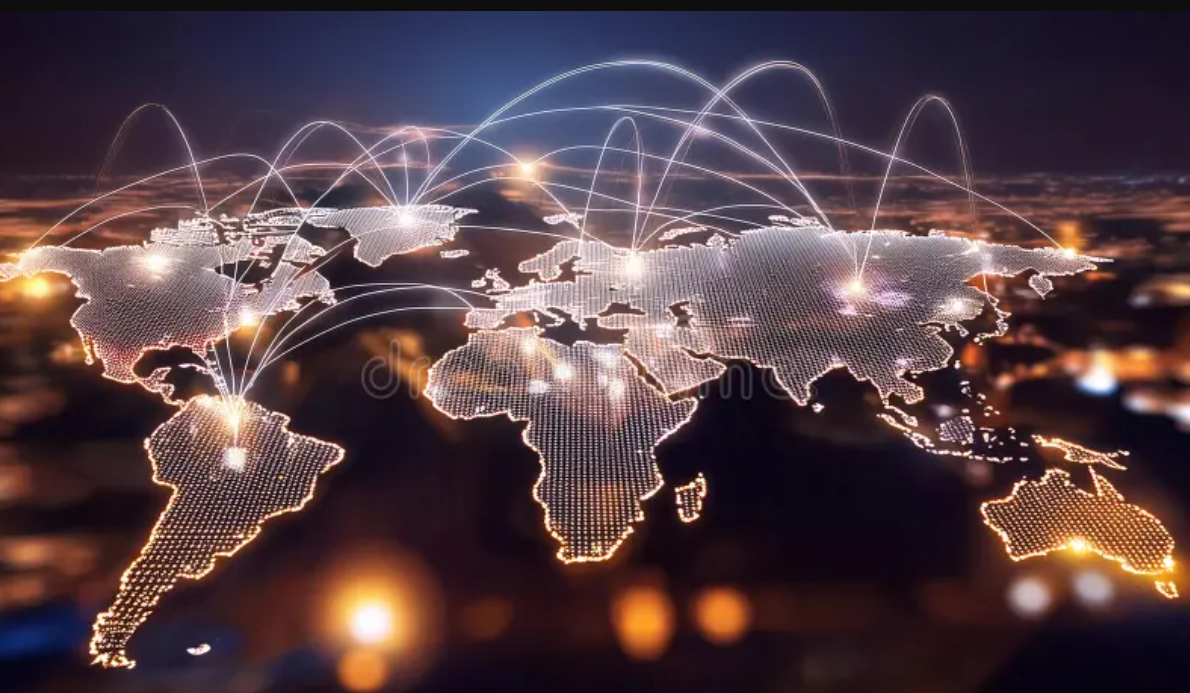
\includegraphics[width=0.45\textwidth]{world.png}
  \caption{\textit{The world is connected, but so are the risks.}}
\end{figure}

\section*{A Light Moment in the Dark Web}
Why did the hacker prefer the dark web? Because the regular internet kept shedding too much light on their plans!

\begin{figure}[h]
  \centering
  
\includegraphics[width=0.45\textwidth]{hacker.png}
  \caption{\textit{A hacker's paradise thrives in the shadows.}}
\end{figure}

\section*{The Worst Cyber Attacks: A Wake-Up Call}
Cyber attacks have left deep scars. Among the worst:

\begin{enumerate}[label=\arabic*.]
  \item \textbf{WannaCry Ransomware (2017)}: Affected 200,000+ systems in 150 countries, including the UK’s NHS. Losses reached £92 million.
  \item \textbf{NotPetya (2017)}: Spread from Ukraine to 60+ countries. Caused \$10 billion in damages, hitting global giants like Maersk and FedEx.
  \item \textbf{Colonial Pipeline (2021)}: Shut down a major US oil pipeline, causing fuel shortages and a \$4.4 million ransom.
\end{enumerate}

\begin{figure}[h]
  \centering
  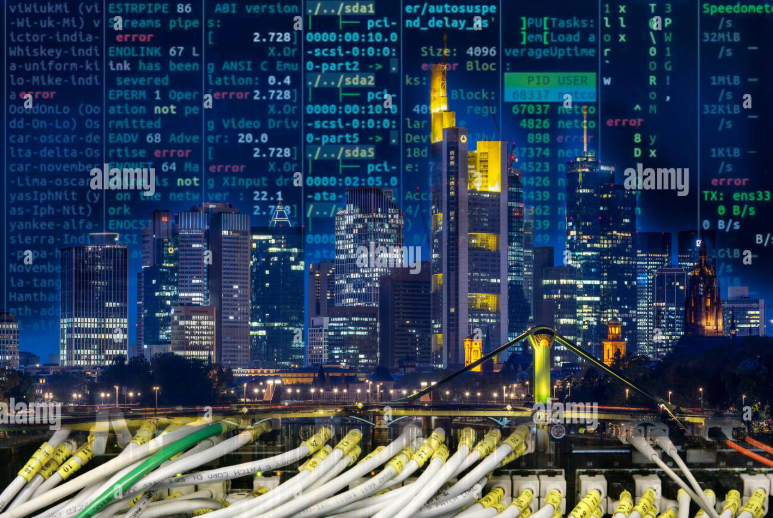
\includegraphics[width=0.45\textwidth]{city.png}
  \caption{\textit{The ripple effects of a cyberattack can paralyze entire systems.}}
\end{figure}

\section*{Vulnerabilities: The Inevitable Weakness}
If there's a vulnerability, it will be exploited. In 2024 alone, 30,000 new vulnerabilities were logged—half high or critical. From unpatched software to weak passwords, cybercriminals exploit them ruthlessly.

\begin{magquote}
``Trust is the ultimate vulnerability in cybersecurity.'' -- Wendy Nather
\end{magquote}

Defense must be proactive. A single misconfigured server or phishing email can compromise entire systems.

\section*{What We Must Do}
To stay secure, we need a multi-layered approach:

\begin{itemize}
  \item \textbf{Education}: 95\% of breaches come from human error.
  \item \textbf{Zero-trust security}: Never assume access is safe.
  \item \textbf{AI-driven defenses}: Can reduce breach costs by millions.
  \item \textbf{Personal hygiene}: Strong passwords, MFA, and software updates.
\end{itemize}

\begin{magquote}
``There's no silver bullet solution with cybersecurity, a layered defense is the only viable defense.'' -- James Scott
\end{magquote}

\begin{figure}[h]
  \centering
  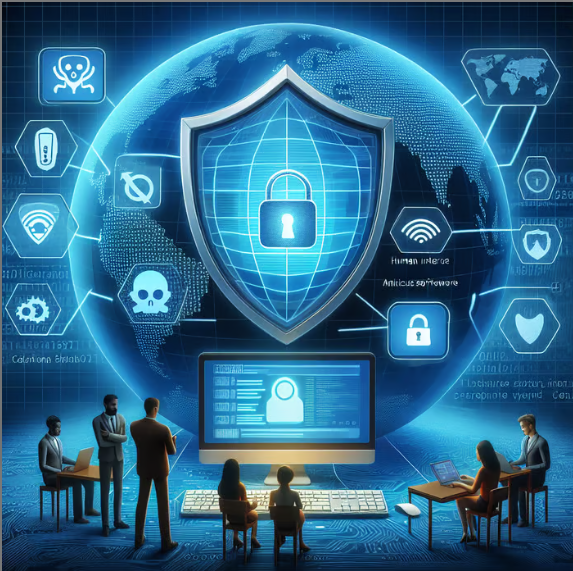
\includegraphics[width=0.45\textwidth]{security.png}
  \caption{\textit{Comprehensive Cyber Defense Strategy.}}
\end{figure}

\section*{The Future of Earth’s Digital Landscape}
Looking ahead, IoT growth (64B devices by 2026) will increase the attack surface. AI-powered attacks will exploit deepfakes and psychology. But quantum-safe encryption and real-time threat detection may level the field.

Still, humans remain the weakest link. Without international cooperation and regulation, cybercrime costs (projected at \$10.5 trillion in 2025) could rise further.

\section*{Sentinel’s Resolve: A Call to Action}
In this digital maze, cybersecurity is not a luxury—it’s a necessity. Let’s embrace education, adopt proactive strategies, and foster global cooperation.

\begin{magquote}
``Cybersecurity is a continuous cycle of protection, detection, response, and recovery.'' -- Chris Painter
\end{magquote}

Let us stand as sentinels, resolute in protecting a future where technology empowers, not endangers.

% PASTE ARTICLE 3 CONTENT HERE
